\documentclass[letterpaper,addpoints,answers]{exam}
\usepackage{graphicx}
\usepackage{multicol}
\usepackage{tikz}

\makeatletter
\def\grd@save@target#1{%
  \def\grd@target{#1}}
\def\grd@save@start#1{%
  \def\grd@start{#1}}
\tikzset{
  grid with coordinates/.style={
    to path={%
      \pgfextra{%
        \edef\grd@@target{(\tikztotarget)}%
        \tikz@scan@one@point\grd@save@target\grd@@target\relax
        \edef\grd@@start{(\tikztostart)}%
        \tikz@scan@one@point\grd@save@start\grd@@start\relax
        \draw[minor help lines] (\tikztostart) grid (\tikztotarget);
        \draw[major help lines] (\tikztostart) grid (\tikztotarget);
        \grd@start
        \pgfmathsetmacro{\grd@xa}{\the\pgf@x/1cm}
        \pgfmathsetmacro{\grd@ya}{\the\pgf@y/1cm}
        \grd@target
        \pgfmathsetmacro{\grd@xb}{\the\pgf@x/1cm}
        \pgfmathsetmacro{\grd@yb}{\the\pgf@y/1cm}
        \pgfmathsetmacro{\grd@xc}{\grd@xa + \pgfkeysvalueof{/tikz/grid with coordinates/major step x}}
        \pgfmathsetmacro{\grd@yc}{\grd@ya + \pgfkeysvalueof{/tikz/grid with coordinates/major step y}}
        \foreach \x in {\grd@xa,\grd@xc,...,\grd@xb}
        \node[anchor=north] at (\x,\grd@ya) {\pgfmathprintnumber{\x}};
        \foreach \y in {\grd@ya,\grd@yc,...,\grd@yb}
        \node[anchor=east] at (\grd@xa,\y) {\pgfmathprintnumber{\y}};
      }
    }
  },
  minor help lines/.style={
    help lines,
    gray,
    line cap =round,
    xstep=\pgfkeysvalueof{/tikz/grid with coordinates/minor step x},
    ystep=\pgfkeysvalueof{/tikz/grid with coordinates/minor step y}
  },
  major help lines/.style={
    help lines,
    line cap =round,
    line width=\pgfkeysvalueof{/tikz/grid with coordinates/major line width},
    xstep=\pgfkeysvalueof{/tikz/grid with coordinates/major step x},
    ystep=\pgfkeysvalueof{/tikz/grid with coordinates/major step y}
  },
  grid with coordinates/.cd,
  minor step x/.initial=.5,
  minor step y/.initial=.2,
  major step x/.initial=1,
  major step y/.initial=1,
  major line width/.initial=1pt,
}
\makeatother


\begin{document}

\begin{coverpages}
 \large\bfseries
 
 \noindent 
 Physics 107: Physics for Life-Sciences

 \vspace{2ex}
 \noindent
 Midterm Exam: October 20, 2014

 \vspace{3ex}
 \noindent 
 This test is administered under the rules and regulations of the honor code of the College of William \& Mary.

 \vspace{2ex}
 \noindent 
 Name:\enspace\makebox[2.3in]{\hrulefill} \\

 \noindent 
 Signature:\enspace\makebox[2in]{\hrulefill} \\

 \vspace{5ex}
 \noindent 
 Instructions:
 \begin{itemize}
  \item This is a closed book, closed notes test.
  \item Calculators are permitted, but not laptops or cell phones. Devices with wireless connections are not allowed.
  \item Start your work from the fundamental equations on the formula sheet, and derive any additional expressions that you may need.
  \item Circle your answer for each part of each problem. 
  \item Clearly mark out any work that you wish the grader to disregard.  Do not waste your time erasing.
  \item Your work will be graded based on your ability to write down a logical and organized solution grounded in the correct assessment of the physics of a situation. No credit will be given for an answer that is not justified by a logical solution or where that justification is not organized or readable. Partial credit will be given up to the point where your solution departs from a correct analysis of the physics involved for any given part of a problem.
 \end{itemize}

 \pagebreak

 \begin{center}
  \gradetable[v][questions]
 \end{center}
 
\end{coverpages}
 

\begin{questions}

\question
Part of riding a bicycle involves leaning at the correct angle when making a turn.  The force exerted by the ground on the wheel can be resolved into two perpendicular components, the force of friction $\vec{f}$ and the normal force $\vec{N}$.  To be in equilibrium the total force exerted by the ground must be on a line through the center of gravity of the bicycle and rider (this requirement imposes a relation between $\vec{f}$ and $\vec{N}$).

\begin{parts}
 \part[5] Draw a free-body diagram of this system, and write down Newton's second law in horizontal and vertical components.
 \vspace{14\baselineskip} 
 \part[10] Determine the angle $\theta$ from the vertical with which the bike will have to lean when you are making a turn at a velocity of 12.0\,m/s with a turn radius of 30.0\,m.  The mass of the bicycle and person is 90\,kg, and the coefficient of static friction of the tire on the road is $\mu_s = 0.9$.
 \vspace{12\baselineskip}
 \part[5] Turns on ice are much more difficult to negotiate than turns on concrete.  If the coefficient of static friction is $\mu_s = 0.05$, what changes in your derivation above?  What is the minimum coefficient of static friction required to negotiate the curve at the velocity and turn radius above?
 \vspace{8\baselineskip}
\end{parts}


\pagebreak

\question
A bungee jumper with a mass of 80\,kg is determining the length of rope necessary for a jump from a 100\,m high bridge (for obvious reasons she does not want to make any mistakes). Assume that the massless rope has a diameter of 1\,cm, an initial length of 80\,m, and a small Young's modulus of $0.002 \times 10^{9}\,$N/m$^2$ (the rope remains in the elastic regime through-out the jump).
\begin{parts}
 \part[5] What is Hooke's constant for the rope?
 \vspace{10\baselineskip}
 \part[5] Using conservation of energy, determine the velocity immediately before the rope starts to stretch.
 \vspace{10\baselineskip}
 \part[10] Using conservation of energy, determine the lowest point the jumper reaches.  Should she use a shorter rope, or does the rope have a safe length?
 \vspace{12\baselineskip}
 \part[5] Draw a free-body diagram at the lowest point and determine the tension in the rope at that point.
 \vspace{10\baselineskip}
\end{parts}


\pagebreak

\question
The objective of curling, an Olympic discipline, is to throw stones at houses. The \emph{stone} is a 20\,kg block of granite that slides on the carefully prepared ice with a very low coefficient of kinetic friction, $\mu_k = 0.0168$. With a curling broom the players can increase the friction to get as close as possible to the \emph{house}, the target pattern embedded in the ice. Frequently an oncoming stone will bump a stone from a previous throw by the competing team.

\begin{center}
 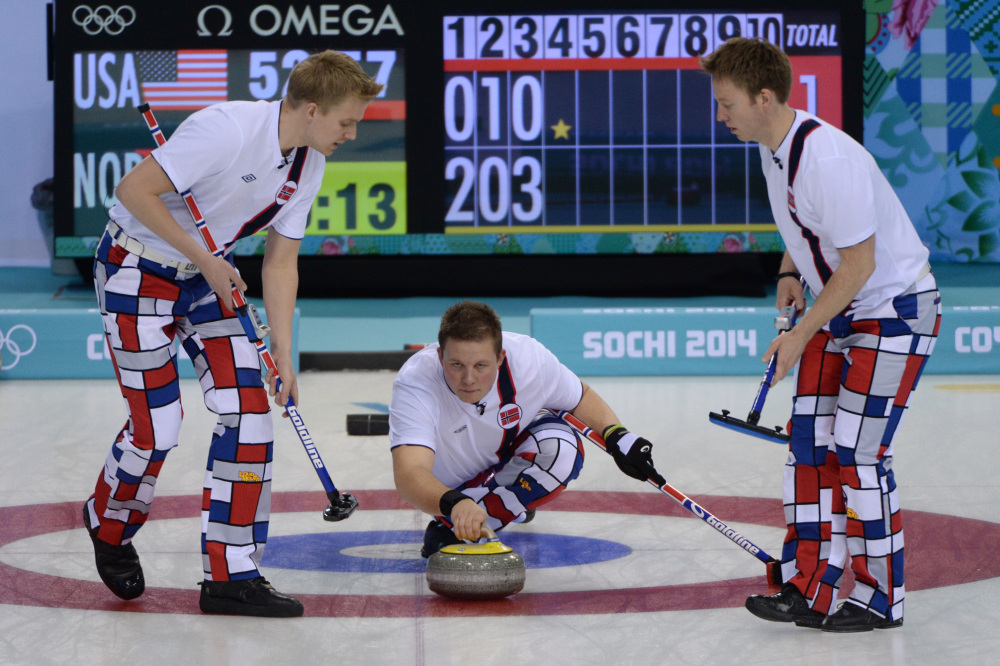
\includegraphics[width=0.6\textwidth]{test2/curling-photo}
\end{center}
\begin{center}
 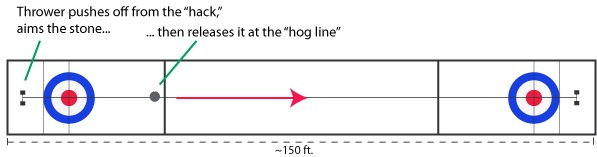
\includegraphics[width=0.6\textwidth]{test2/curling-sheet}
\end{center}

\begin{parts}
 \part[10] An stone reaches the house with a velocity of 1\,m/s after traveling the 40\,m length of the curling lane. Assuming a constant coefficient of friction, use conservation of energy to determine how fast the stone was going when it was released.
 \vspace{8\baselineskip}
 
 \part[10] The oncoming stone with a velocity $v_1$ of 1\,m/s bumps a second motionless stone head-on. What are the velocities $v_1$ and $v_2$ of the two stones after this elastic collision?
 \vspace{10\baselineskip}
 
 \part[5] In a bad throw the stone with a velocity of 1\,m/s bounces perpendicularly of the back end wall of the lane and returns with a velocity of 0.5\,m/s. What is the average force of the stone on the wall if the collision lasted for 30\,ms?
 \vspace{6\baselineskip}
 
\end{parts}


%In an attempt to develop a new Olympic discipline, the Canadian and American teams have decided to join forces: softball on ice!  A softball has a mass of 200 g is launched horizontally by the pitching machine with a velocity of 30 m/s. The batter at the edge of the ice arena gives it a horizontal impulse of $5\,\hbox{N} \cdot \hbox{s}$ and a vertical impulse of $4\,\hbox{N} \cdot \hbox{s}$. A skater on the frictionless ice surface catches the ball and holds on to it while she recoils. While she is recoiling, the skater throws the ball to the 

\end{questions}

 \pagebreak
 
 {\Large Possibly useful relations (feel free to detach this page):}
  
 \fontseries{\seriesdefault}
 \begin{multicols}{2}
 \Large
 \noindent
 $\vec{v}_{avg} = \Delta\vec{x} / \Delta t$ \\
 $x = x_0 + v_0 t + \frac{1}{2} a t^2$ \\
 $v^2 = v_0^2 + 2 a (x - x_0)$ \\
 $R = \frac{v_0^2}{g}\sin 2\theta$ \\
 $\vec{F}_{net} = m \vec{a}$ \\
 $\vec{W} = m \vec{g}$ \\
 $\vec{g} = 9.80\,$m/s$^2$ downward \\
 $\cos\theta = \hbox{adjacent}/\hbox{hypotenuse}$ \\
 $\sin\theta = \hbox{opposite}/\hbox{hypotenuse}$ \\
 $\frac{F}{A} = Y \frac{\Delta L}{L}$ \\
 $W = F d \cos\theta$ \\
 $W_{\hbox{net}} = -\Delta PE$ \\
 $PE_k = \frac{1}{2} k x^2$ \\
 $PE_g = m g h$ \\
 $KE_i + PE_i + W_{nc} = KE_f + PE_f$ \\
 $\hbox{Eff} = \frac{W_{out}}{E_{in}}$ \\
 $\vec{p} = m \vec{v}$ \\
 $\theta = \frac{s}{r}$ \\
 $v = r \omega$ \\
 $f = \frac{1}{T}$ \\
 $1\,\hbox{cal} = 4.186$\,J \\ 
 $1\,\hbox{Cal} = 1000$\,cal \\ 

 \noindent
 $\vec{a}_{avg} = \Delta\vec{v} / \Delta t$ \\
 $v = v_0 + a t$ \\
 $v_{avg} = \frac{v_0 + v}{2}$ \\
 $h = \frac{v_0^2}{2 g} \sin^2 \theta$ \\
 $\vec{F}_{BA} = - \vec{F}_{AB}$ \\
 $0 \le f_s \le \mu_s N$ \\
 $f_k = \mu_k N$ \\
 $\tan\theta = \sin\theta / \cos\theta$ \\
 $x = \frac{-b \pm \sqrt{b^2 - 4 a c}}{2 a}$ \\
 $F_k = -k x$ \\
 $KE = \frac{1}{2} m v^2$ \\
 $W_{\hbox{net}} = \Delta KE$ \\
 $P = \frac{W}{\Delta t}$ \\
 $\vec{I} = \vec{F}_{avg} \Delta t$ \\
 $\vec{F}_{net} = \frac{\Delta \vec{p}}{\Delta t}$ \\
 $v_1 - v_2 = v'_2 - v'_1$ \\
 $F_c = m\frac{v^2}{r} = m r \omega^2$ \\
 $\omega = \frac{\Delta \theta}{\Delta t}$ \\
 $a_c = \frac{v^2}{r} = r \omega^2$ \\
 $\omega = 2 \pi f$ \\
 $F = G \frac{m M}{r^2}$ \\
 $G = 6.67 \times 10^{-11}\,$N $\cdot$ m$^2$ / kg$^2$ \\
  
 \end{multicols}

\end{document}
